

\subsection{Model 1: Non-Speech Liability}

There are two distinctive features of platform liability for third-party speech: it involves liability for \emph{speech} rather than conduct, and it involves liability for the speech of \emph{others} rather than the platform's own speech. Both of these features are essential to the economic case for intermediary immunity. To see why, it is useful to start with a model in which they are absent.

We start with a model of a non-speech first-party actor. A widget factory chooses its level of production from the interval $[0,n]$. It has a constant marginal revenue $P$ per unit of widgets produced. But as its level of production increases, it must resort to increasingly harmful techniques to make its production target. Let the marginal harms from the factory's pollution be $h(x)$ for $x \in [0,n]$, where $h(x)$ is a weakly increasing function (i.e. $x < y$ implies $h(x) \le h(y)$). For simplicity of exposition, we assume that initial production is completely harmless (i.e. $h(0) =0$). Then the following simple diagram illustrates social welfare as a function of the factory's output:\footnote{In the case where $h(n) < P$, the curves $h(x)$ and $P$ never intersect, and both the socially optimal and privately optimal behavior is for the factory to maximize production.}
\begin{figure}[h]
    \centering
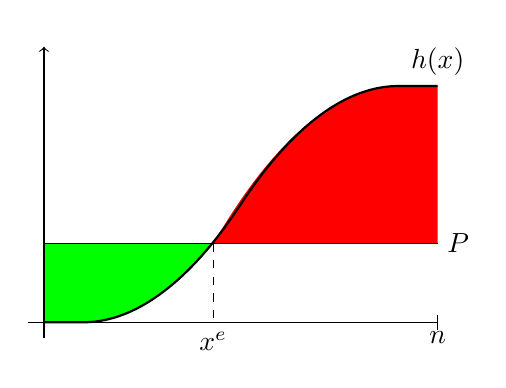
\begin{tikzpicture}[scale=1]
    \fill[green] (0,0) to (.5,0) parabola (2.15,1) to (0,1) to (0,0);
    \fill[red] (2.15,1) parabola[bend at end] (4.5,3) to (5,3) to (5,1) to (2,1);
    \draw[-|] (-0.2,0) -- (5,0) node[below]{$n$}; 
    \draw[->] (0,-0.2) -- (0,3.5) node[above]{};
    \draw[thick] (0,0) to (.5,0) parabola (2.5,1.5) parabola[bend at end] (4.5,3) to (5,3) node[above]{$h(x)$};

    \draw[thin] (0,1) to (5,1) node[right]{$P$};
    \draw[dashed, thin] (2.15,1) -- (2.15,0) node[below]{$x^e$}; 

%    \draw[thin] (0,2) to (5,2) node[right]{$S+P$};
%    \draw[dashed, thin] (1.75,1.5) -- (1.75,0) node[below]{$x^p$}; 
    
%    \draw[thin] (0,3) to (5,3) node[right]{$S+P+L$};
%    \draw[dashed, thin] (3.55,3) -- (3.55,0) node[below]{$x^e$}; 
    
\end{tikzpicture}
    \caption{Non-Speech Torts}
    \label{fig:nonspeech}
\end{figure}
The net benefit or harm to society from the factory's production at $x$ is given between the signed difference between $P$ and $h(x)$. Production in the green region, where $P > h(x)$ is net beneficial. Although there are harms from pollution, they are outweighed by the value of the corresponding widgets. Production in the red region, where $P < h(x)$, is net harmful. Here, the harms from pollution are worse than the value of the corresponding widgets; society would be better off if these widgets were not produced at all. If that the factory produces up to a level $\hat{x}$, social welfare will be given by:
\begin{equation}
\int_{0}^{\hat{x}} P - h(x) dx
\end{equation}
It is easy to see that the efficient outcome is when the factory produces just up to the threshold $x^e$ defined by $h(x^e) = P$. At $x_e$, all of the beneficial widgets and none of the harmful widgets are produced. The question is how to get there. Write $x^{\ast}$ for the production level that maximizes the factory's profits, and consider the following legal regimes:
\begin{itemize}
\item \textbf{No liability}: If the factory faces no liability for the pollution it causes, it will set $x^{\ast} = n$, making a profit of $nP$. But since $n > x^e$, social welfare will be less than the efficient level, and may even (as in the diagram above) be negative.
\item \textbf{Prohibition}: If society bans widgets, the factory will set $x^{\ast} = 0$ and make a profit of $0$. But since $0 < x^e$, social welfare will be less than the efficient level. For some values of $h$ and $P$, prohibition will be better than no liability; for other values, it will be worse.
\item \textbf{Strict Liability}: If the factory is forced to pay compensation for all of the harms that it causes, the factory's marginal profit will be $P - h(x)$, which is identical to the social welfare function. The factory's marginal profit will become zero at $x^e$, exactly when social welfare does. Thus $x^{\ast} = x^e$ and the factory will act efficiently.
\end{itemize}
This is the standard law-and-economics case for strict liability. But one of its essential assumptions fails when the product is not widgets, but speech.


\subsection{Model 2: Speech Liability}

Speech consists of information, and information is a public good. Once it has been shared with one listener, the speaker cannot easily prevent them from sharing it with others.\footnote{Arrow, Lemley, Frischmann, Baker} This third-party value is an externality from the speaker's perspective. 

We model this externality by adding an additional term $\delta > 0$ to the value created by carrying a given piece of content. Like $P$, we assume that $\delta$ is constant across all content. Thus, while each unit of widget production generates $P$ in marginal profit for the factory, each unit of speech generates $P$ in value for the speaker and $\delta$ in value for society at large, for a total of $P + \delta$. Now the diagram looks like:\footnote{Again, if $h(n) < P + \delta$, the curve $h(x)$ will fail to intersect one or both of $P$ and $P + \delta$. In these cases, it is socially optimal to maximize speech production, and both negligence law and no liability are efficient.}
\begin{figure}[h]
    \centering
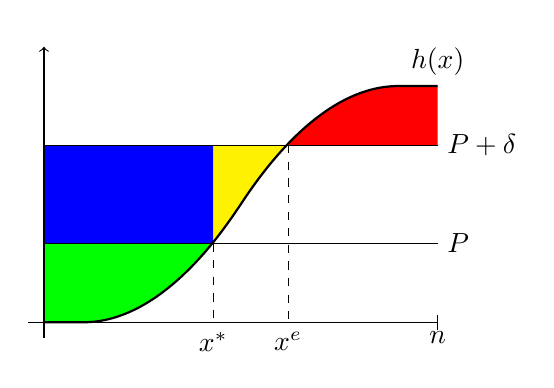
\begin{tikzpicture}[scale=1]
    \fill[green] (0,0) to (.5,0) parabola (2.15,1) to (0,1) to (0,0);
    \fill[red] (3.1,2.25) parabola[bend at end] (4.5,3) to (5,3) to (5,2.25) to (3.1,2.25);
    \fill[blue] (0,1) to (2.15,1) to (2.15,2.25) to (0,2.25) to (0,1);
    \fill[yellow] (2.15,1) parabola bend +(-1.65,-1) (2.5,1.5) parabola bend +(2,1.5) (3.1,2.25) to (2.15,2.25) to (2.15,1);
    \draw[-|] (-0.2,0) -- (5,0) node[below]{$n$}; 
    \draw[->] (0,-0.2) -- (0,3.5) node[above]{};
    \draw[thick] (0,0) to (.5,0) parabola (2.5,1.5) parabola[bend at end] (4.5,3) to (5,3) node[above]{$h(x)$};

    \draw[thin] (0,1) to (5,1) node[right]{$P$};
    \draw[dashed, thin] (2.15,1) -- (2.15,0) node[below]{$x^*$}; 

    \draw[thin] (0,2.25) to (5,2.25) node[right]{$P+\delta$};
    \draw[dashed, thin] (3.1,2.25) -- (3.1,0) node[below]{$x^e$}; 
    
%    \draw[thin] (0,3) to (5,3) node[right]{$S+P+L$};
%    \draw[dashed, thin] (3.55,3) -- (3.55,0) node[below]{$x^e$}; 
    
\end{tikzpicture}
    \caption{Speech Torts}
    \label{fig:speech}
\end{figure}
The efficient level of speech $x^e$ is defined not by where $h(x)$ intersects the speaker's marginal profit curve $P$ but by where it intersects society's marginal benefit curve $P+\delta$. Under no liability, the speaker will still overproduce (producing the net-harmful speech in the red area); under prohibition, the speaker will still underproduce (failing to produce the net-beneficial speech in the green and blue areas) . But now also strict liability gets the incentives wrong. Under strict liability, the speaker will produce speech up to $x^*$ where $h(x^*) = P$. But because $P + \delta > P$ and $h(x)$ is a weakly increasing function, $x^* \le x^e$. Pictorially, the platform will produce up to $x^*$, generating profits in the green region and spillover social benefits in the blue region. But there it will stop, even though the speech from $x^*$ to $x^e$ would have been beneficial to society: the yellow region represents foregone social welfare. \footnote{Strict liability is strictly better than prohibition, which also gives up the green and blue regions. Whether strict liability is better than full immunity is indeterminate without more constraints on $h(x)$, $P$, and $\delta$; the yellow region could be larger than the red, or vice versa.}

Instead, free speech law typically follows the negligence strategy of defining an objective standard of care that a reasonable person is expected to follow when acting. One who acts according to that standard of care faces no liability, even if others are harmed. But one who fails to meet that standard is held liable for the resulting harms. In our model, this approach corresponds to defining a threshold of liability $t$ and subjecting the actor to marginal liability:
\begin{equation}
\lt\{\begin{array}{ll}
    0 & \mbox{for $x <t$}, \\
    h(x) & \mbox{for $x \ge t$}.
\end{array}\rt.
\end{equation}
It is easy to see that if the threshold is set at $t=x^e$, then the actor's incentives again align with social welfare.\footnote{Cooter, prices and sanctions} This is a standard argument for treating speech torts differently than other types of torts. Because the speaker creates value for listeners and for society by spreading information, the value of the speech \emph{to them} must be weighed against the harm that it causes. Thus, harmful true speech is frequently protected (e.g. negative consumer reviews). Similarly, the public-disclosure tort contains a First-Amendment-driven exception when the information is of legitimate public concern, i.e., when $\delta$ is high.

This model explains why speech law is more solicitous of speakers than of other actors. But notice that it cannot yet explain why speech law is even more solicitous of platforms than it is of speakers! The spillover critique of strict liability applies just as strongly to original speakers as it does to platforms. And the negligence strategy suggests that the threshold of liability should be based entirely on the overall \emph{social} costs and benefits of the speech: whatever that threshold is, it should apply equally to speakers and platforms, regardless of their private incentives. Something further is required to make sense of platform immunity.


\subsection{Model 3: Imperfect Information About Speech}

Individual speakers post content to a platform. The platform can choose whether to allow each item of content to remain up or to take it down. Each unit of content generates $ \ge 0$ in private value for the speaker, $P \ge 0$ in private value for the platform, and externality $\delta \ge 0$ for society at large.

But now we add a second dimension: each item of content is a pair $(x,y)$.  The $x$ axis measures harmfulness $h(x)$, as before. But the $y$ axis, which ranges from $0$ to $m$, measures the \emph{fraction} of content that is harmful. That is, for content at $(x,y)$, a fraction $\lambda(y)$ of that content is harmful and generates harm $h(x)$ per unit and a fraction $ 1- \lambda(y)$ is harmless and generates $0$ harm. The speaker of an item of content knows whether it is harmful or not, as does the regulator, but the platform does not. Instead, the platform observes the \emph{probability} $\lambda(y)$ that the item is harmful, where $\lambda(y)$ is a weakly increasing function of $y$, with $\lambda(0) = 0$. That is, the harmfulness $h(x,y)$ of content $(x,y)$ is given by:
\begin{equation}
h(x,y)=
\lt\{\begin{array}{ll}
    h(x) & \mbox{with probability $\lambda(y)$}, \\
    0 & \mbox{with probability $1 - \lambda(y)$}.
\end{array}\rt.
\end{equation}
In expectation, a unit of content at $y$ will generate harm $\lambda(y)h(x)$. Start by examining the platform's incentives. Hold $x$ fixed (so that $h(x)$ is constant and consider the following diagram of benefits and harms as as a function of $y$:
\begin{figure}[h]
    \centering
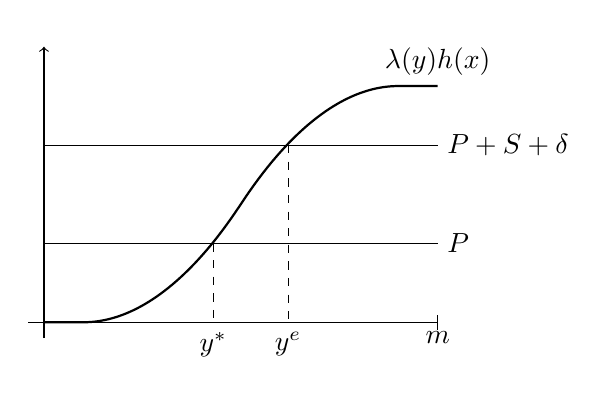
\begin{tikzpicture}[scale=1]
%    \fill[green] (0,0) to (.5,0) parabola (2.15,1) to (0,1) to (0,0);
%    \fill[red] (3.1,2.25) parabola[bend at end] (4.5,3) to (5,3) to (5,2.25) to (3.1,2.25);
%    \fill[blue] (0,1) to (2.15,1) to (2.15,2.25) to (0,2.25) to (0,1);
%    \fill[yellow] (2.15,1) parabola bend +(-1.65,-1) (2.5,1.5) parabola bend +(2,1.5) (3.1,2.25) to (2.15,2.25) to (2.15,1);
    \draw[-|] (-0.2,0) -- (5,0) node[below]{$m$}; 
    \draw[->] (0,-0.2) -- (0,3.5) node[above]{};
    \draw[thick] (0,0) to (.5,0) parabola (2.5,1.5) parabola[bend at end] (4.5,3) to (5,3) node[above]{$\lambda(y)h(x)$};

    \draw[thin] (0,1) to (5,1) node[right]{$P$};
    \draw[dashed, thin] (2.15,1) -- (2.15,0) node[below]{$y^*$}; 

    \draw[thin] (0,2.25) to (5,2.25) node[right]{$P+S+\delta$};
    \draw[dashed, thin] (3.1,2.25) -- (3.1,0) node[below]{$y^e$}; 
    
%    \draw[thin] (0,3) to (5,3) node[right]{$S+P+L$};
%    \draw[dashed, thin] (3.55,3) -- (3.55,0) node[below]{$x^e$}; 
\end{tikzpicture}
    \caption{Speech Torts with Imperfect Information}
    \label{fig:speechimperfect}
\end{figure}
Observe that the curve $\lambda(y)$ has \emph{exactly the same shape} as $h(x)$ did in the previous diagram. We have replaced a deterministic but variable harm $h(x)$ with a probabilistic but fixed harm $\lambda(y)h(x)$. This means that the analysis from the previous model carries over: if the platform chooses to allow content $y$ to remain up, it generates private value $P$ per unit, social value $P+S+\delta$ per unit, and \emph{expected} harm $h(x,y) = \lambda(y)h(x)$ per unit. As long as the platform's potential liability is a weakly increasing function in $y$, it will choose a threshold $\hat{y}$ that maximizes its profits by taking down all content $y > \hat{y}$ beyond the threshold and leaving up all content $y \le \hat{y}$. And as before, there is a socially efficient choice $y^e$, determined by $\lambda(y^e) = \frac{P + S+ \delta}{H}$, at which the platform takes up all and only that content whose expected harms exceed its social value. 

As before, complete immunity leads to undermoderation because the platform sets $\hat{y} = m$, allowing expected net-harmful content to remain. Prohibition leads to overmoderation because the platform sets $\hat{y} = 0$, taking down expected net-beneficial content. Strict liability leads the platform to overmoderate (although less than for prohibition) because the platform sets $\hat{y} = y^{\ast}$ defined by $\lambda(y^{\ast} = \frac{P}{H})$, and $y^{\ast} \le y^e$. Threshold liability is efficient when the threshold is set at $y^e$. The regulator takes into account the value to speakers and society at large of speech.

What is different about this model is that the \emph{platform}'s incentives are different than the \emph{speaker}'s. In particular, because speakers have perfect information along the $y$ axis about whether their content is harmful or not, they have an option the platform does not: to omit the harmful speech while still producing the harmless speech. Because the platform only observes $\lambda(y)$, a noisy signal of the speech's harmfulness, it must remove both harmful and harmless content that have the same $\lambda(y)$.

Observe that \emph{along the $x$ axis of harmfulness}, the regulator's optimal behavior towards speakers \emph{is unchanged}. Strict liability is inefficient in the range $S < h(x) < P + S + \delta$, but threshold liability at $x^e$ defined by $h(x^e) = P + S + \delta$ is socially optimal. The regulator takes into account the value to the platform and to society at large.

In other words, \emph{platform immunity rests on a related but distinct basis than speaker protections}. Both of them depend on positive externalities: when $\delta = 0$, the argument for a more speech-protective regime than strict liability collapses. But the pure speaker-protective argument is that some speech is valuable \emph{notwithstanding} the harms it causes, while the platform-protective argument is that some valuable speech is \emph{indistinguishable} from harmful speech.

There are also good reasons to believe that in typical cases, the value $P$ extracted by a platform is significantly smaller than the value $S$ realized by the users who post content. Estimates of the net social utility created for platform users vastly exceed estimates of the platforms' revenues. This means that in practice, platforms have significantly weaker private incentives to host speech than orignal speakers do. Strict liability more significantly deters platforms than speakers.

\subsection{Model 4: Platform Investigations}


